\documentclass{slide}

\title{Architectural Views}
\subtitle{Software Architecture}
\author{Richard Thomas}
\date{\week{1}}

\usepackage{languages}
\usepackage{changepage}

\usepackage{tikz}
\usetikzlibrary{positioning}
\usetikzlibrary{fit}
\usetikzlibrary{arrows.meta}

\begin{document}

\maketitle

\point[\LARGE\highlight{Interesting} Software is Complex]{Many aspects to the design of its architecture.}

\point[\LARGE{Architectural Design}]{Managing technical complexity.}

\questionanswer{How do you describe a complex architecture, without making it too difficult to understand?}
{\highlight{Architectural Views}\\~~~~ -- Only consider one aspect at a time.}


\begin{frame}{Architectural Views}
\begin{adjustwidth}{-0.5em}{-1em}
\vspace{3mm}
\Large{
\begin{itemize}
    \item<1-> C4 Model \cite{brown2022c4}
    \begin{itemize}
        \large{\item[$-$] context, structure, behaviour, infrastructure}
    \end{itemize}
    \vspace{2mm}
    \item<2-> 4+1 Views \cite{4+1-model}
    \begin{itemize}
        \large{\item[$-$] logical, process, development, physical, scenario}
    \end{itemize}
    \vspace{2mm}
    \item<3-> Software Architecture in Practice \cite{bass2021software}
    \begin{itemize}
        \large{\item[$-$] module, component-and-connector, allocation}
    \end{itemize}
    \vspace{2mm}
    \item<4-> NATO Architecture Framework \cite{nafv4}
    \begin{itemize}
        \large{\item[$-$] concepts, service, logical, physical resource, architecture foundation}
    \end{itemize}
    \vspace{2mm}
    \item<5-> The Open Group Architecture Framework (TOGAF) \cite{togaf}
    \vspace{2mm}
    \item<5-> ISO/IEC/IEEE 42010:2011 \cite{iso42010}
\end{itemize}
}
\end{adjustwidth}
\end{frame}


\begin{frame}{Diagrams \& Notation}

\Large{
\begin{itemize}
    \item<1-> A \highlight{good} diagram is worth a thousand words
    \begin{itemize}
        \large{\item A thousand diagrams is just confusing}
    \end{itemize}
    \vspace{5mm}
    \item<2-> C4 -- informal, simple structure \cite{brown2022c4}
    \vspace{2mm}
    \item<2-> UML -- formal, well-defined language \cite{uml}
    \vspace{3mm}
    \item<2-> You probably don't want to know about alternatives
\end{itemize}
}

\end{frame}


\begin{frame}{C4 Model: Levels}
	\centering
    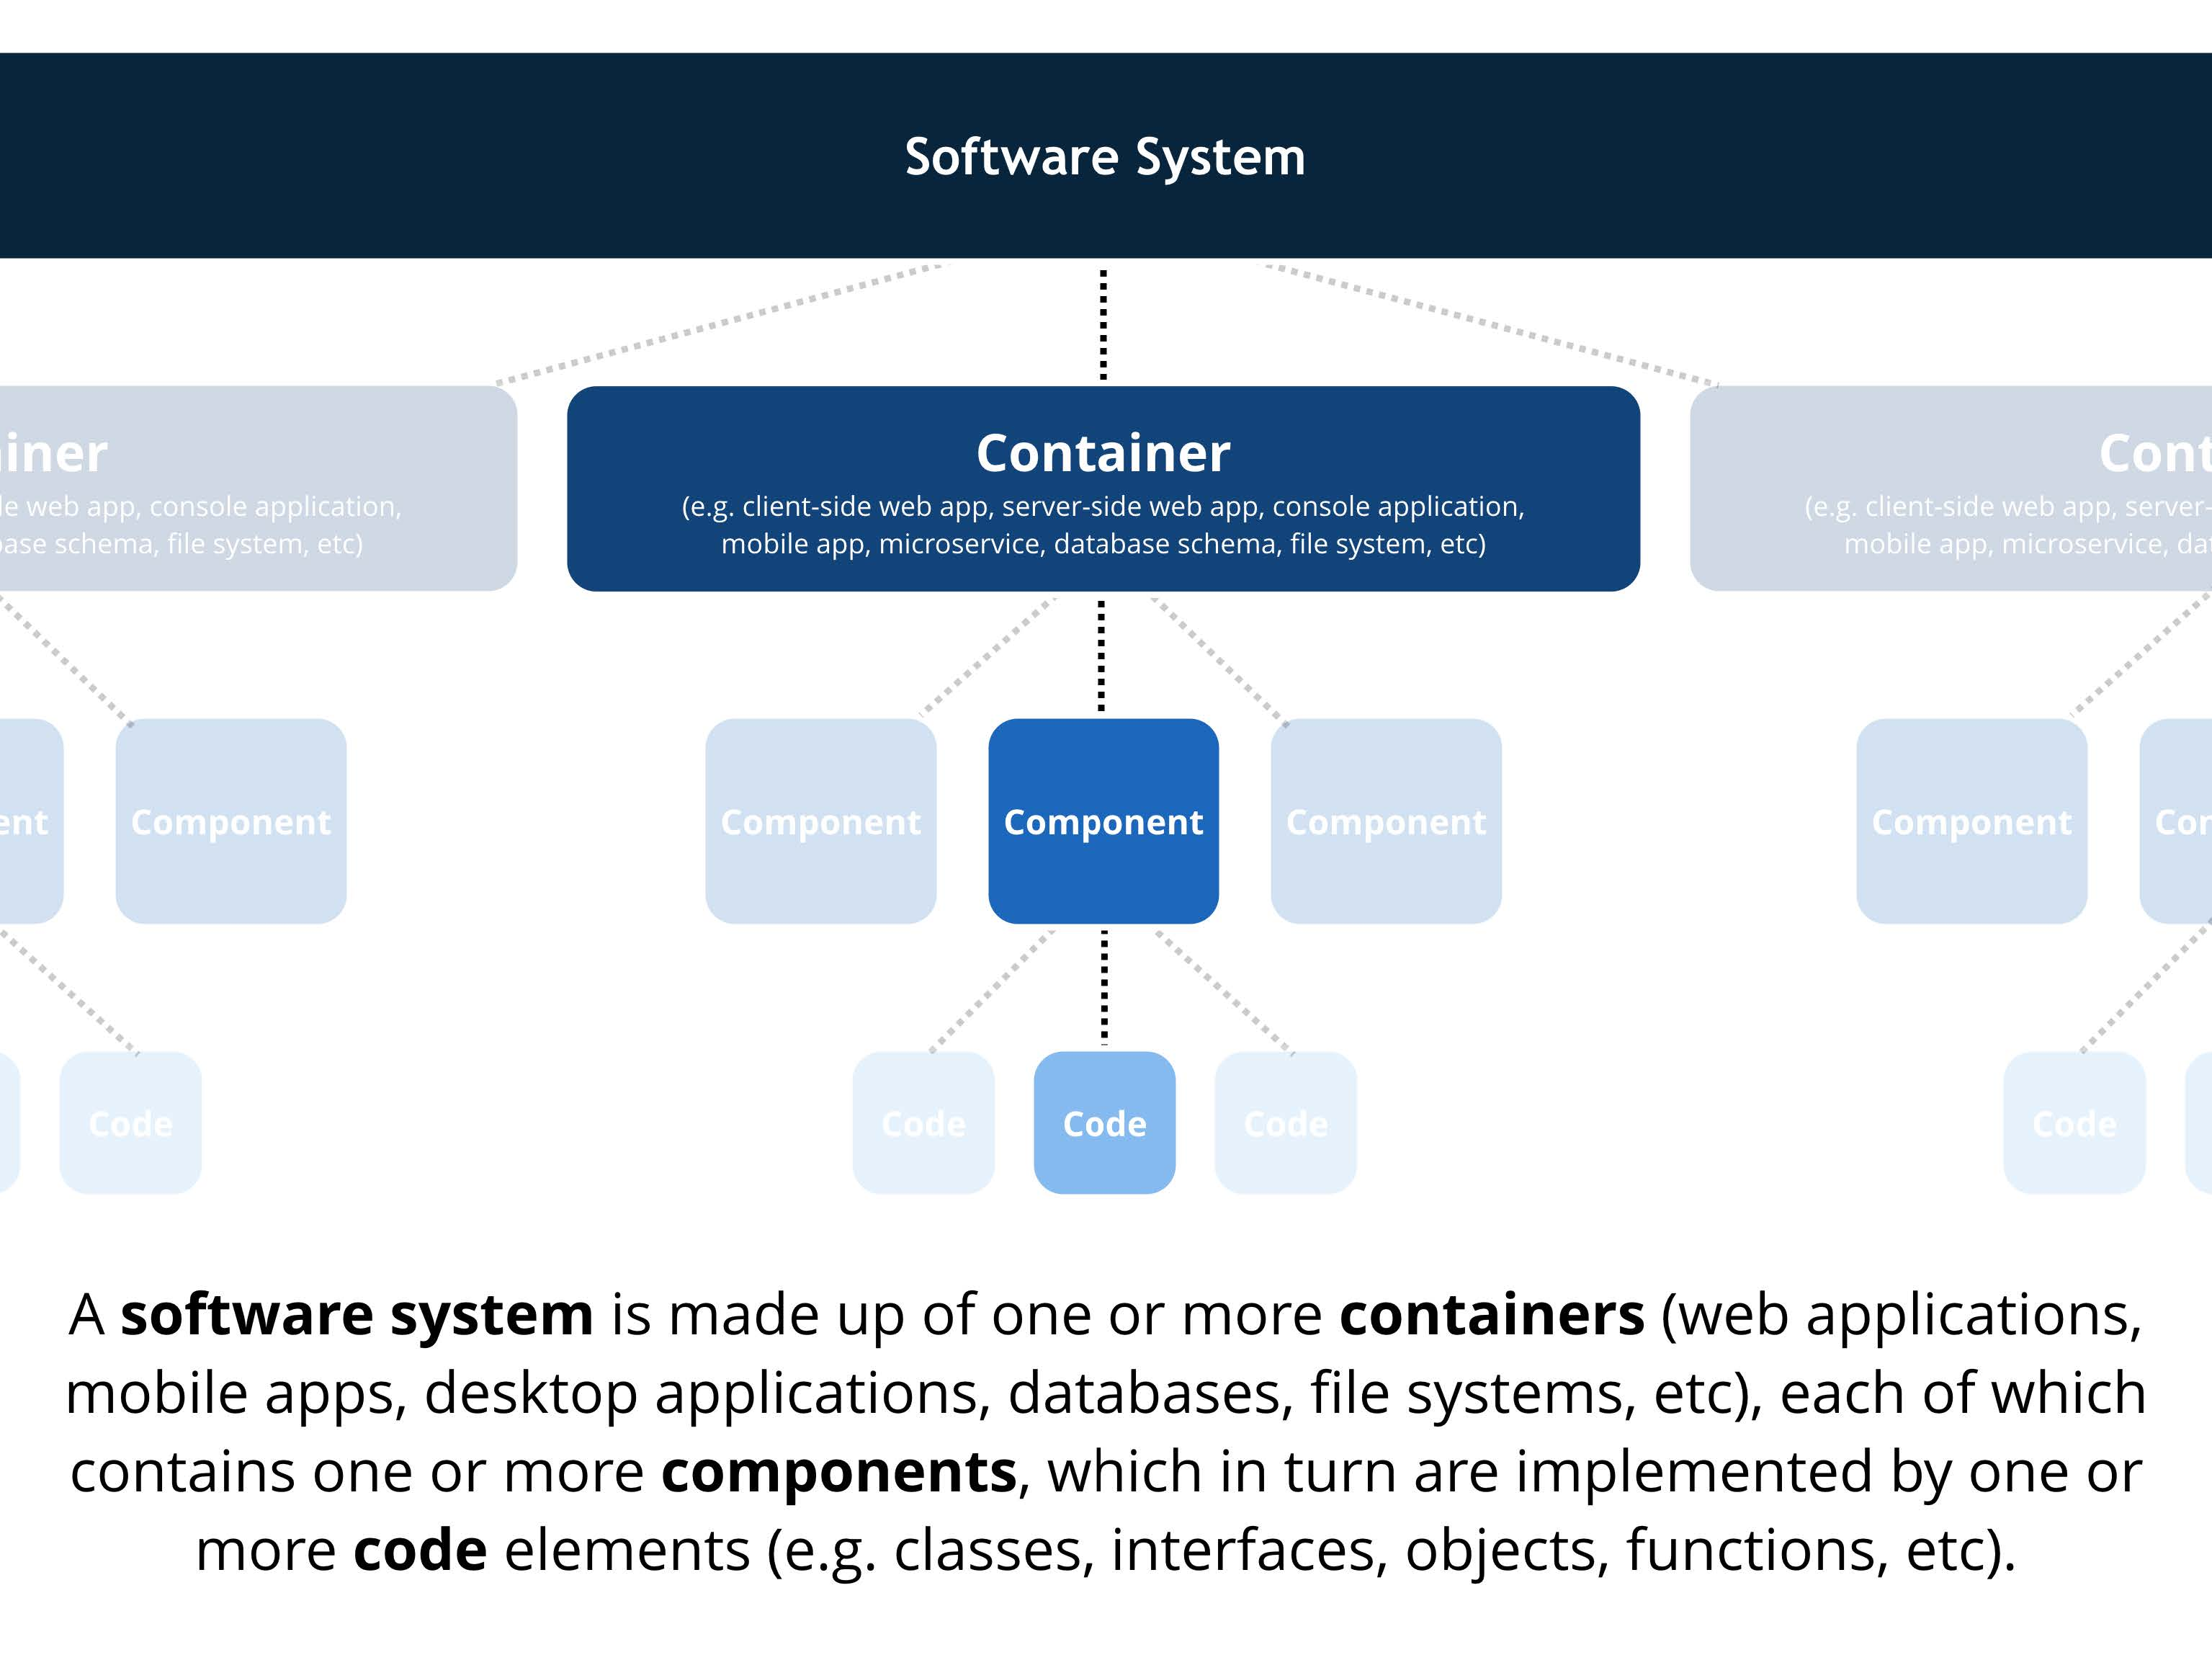
\includegraphics[trim=0 50 0 0,clip,width=0.88\paperwidth]{../../notes/views/images/c4_terminology.jpg}
\end{frame}
\note[itemize]{
    \item \highlight{Software} system is made up of one or more
    \item \highlight{Containers} (web/mobile/desktop apps, dbs, file systems, ...),
    \item each of which contains one or more
    \item \highlight{Components}, which in turn are implemented by one or more
    \item \highlight{Code elements} (classes, interfaces, objects, functions, ...)
}


\begin{frame}{C4 Model: Context}
	\centering
    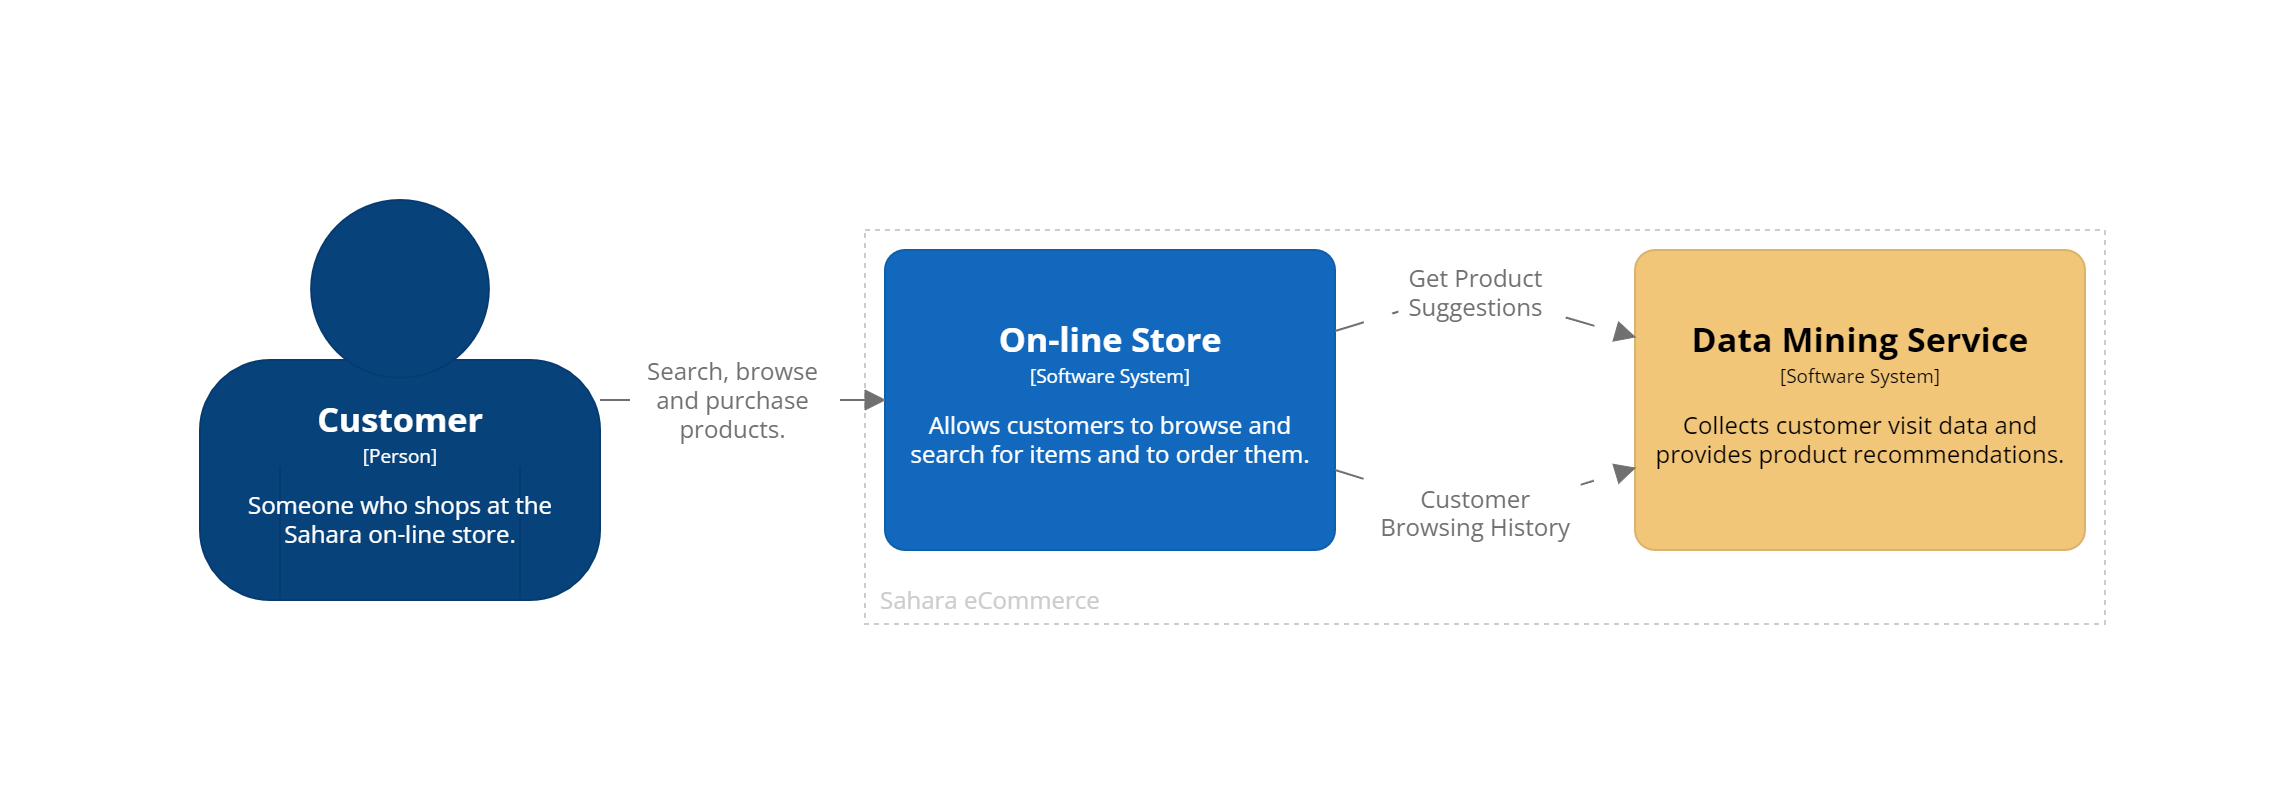
\includegraphics[trim=195 195 198 195,clip,width=0.75\paperwidth]{../../notes/views/images/c4/context_diagram.png}
    
    \vspace{1cm}
    \LARGE{How software system fits into broader \highlight{environment}}
\end{frame}


{
\usebackgroundtemplate{\centerline{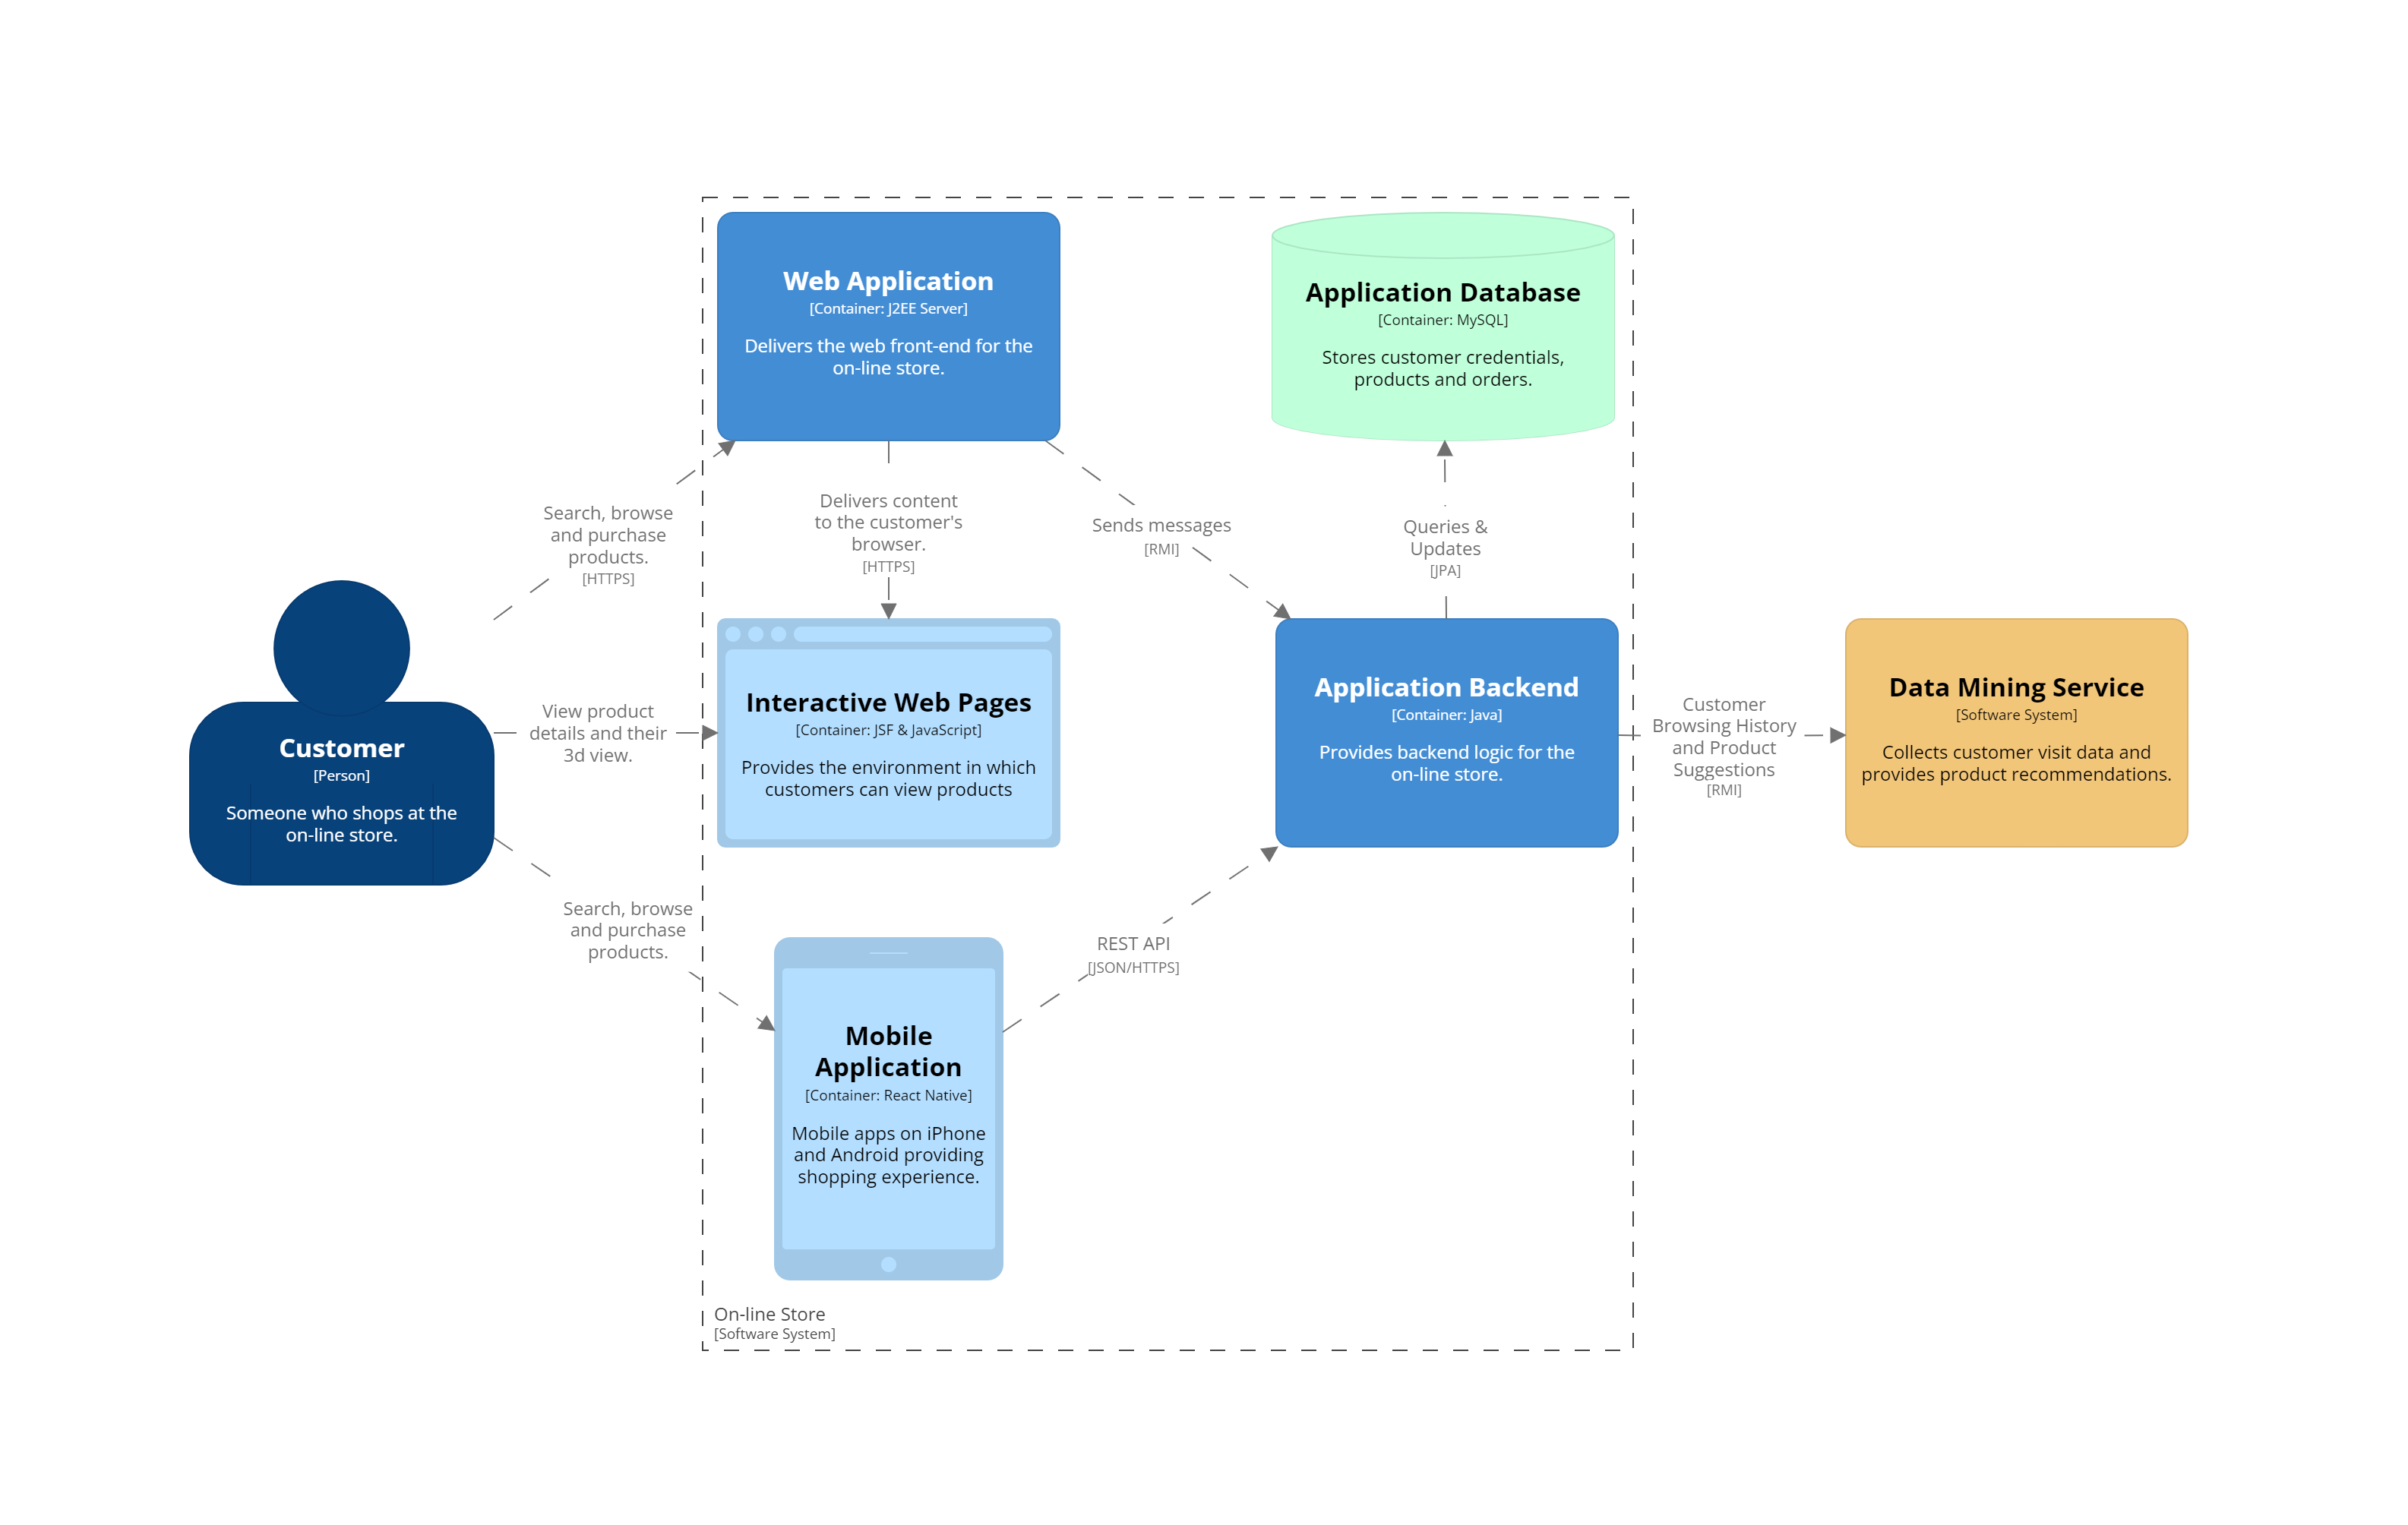
\includegraphics[trim=-475 190 200 70,clip,width=0.96\paperwidth]{../../notes/views/images/c4/store_container_diagram.png}}}
\begin{frame}{C4 Model: Containers}
    \centering
    \vspace{68mm}
    \LARGE{\highlight{Structure} of the software system}
\end{frame}
}
\note[itemize]{
    \item \highlight{Overview} of the architecture
    \item \highlight{Structure} of the software system
    \item \highlight{Technologies} to implement it
    \item \highlight{Deployable} software elements,
    \item web/mobile/desktop apps, dbs, file systems, ...
}


{
\usebackgroundtemplate{\centerline{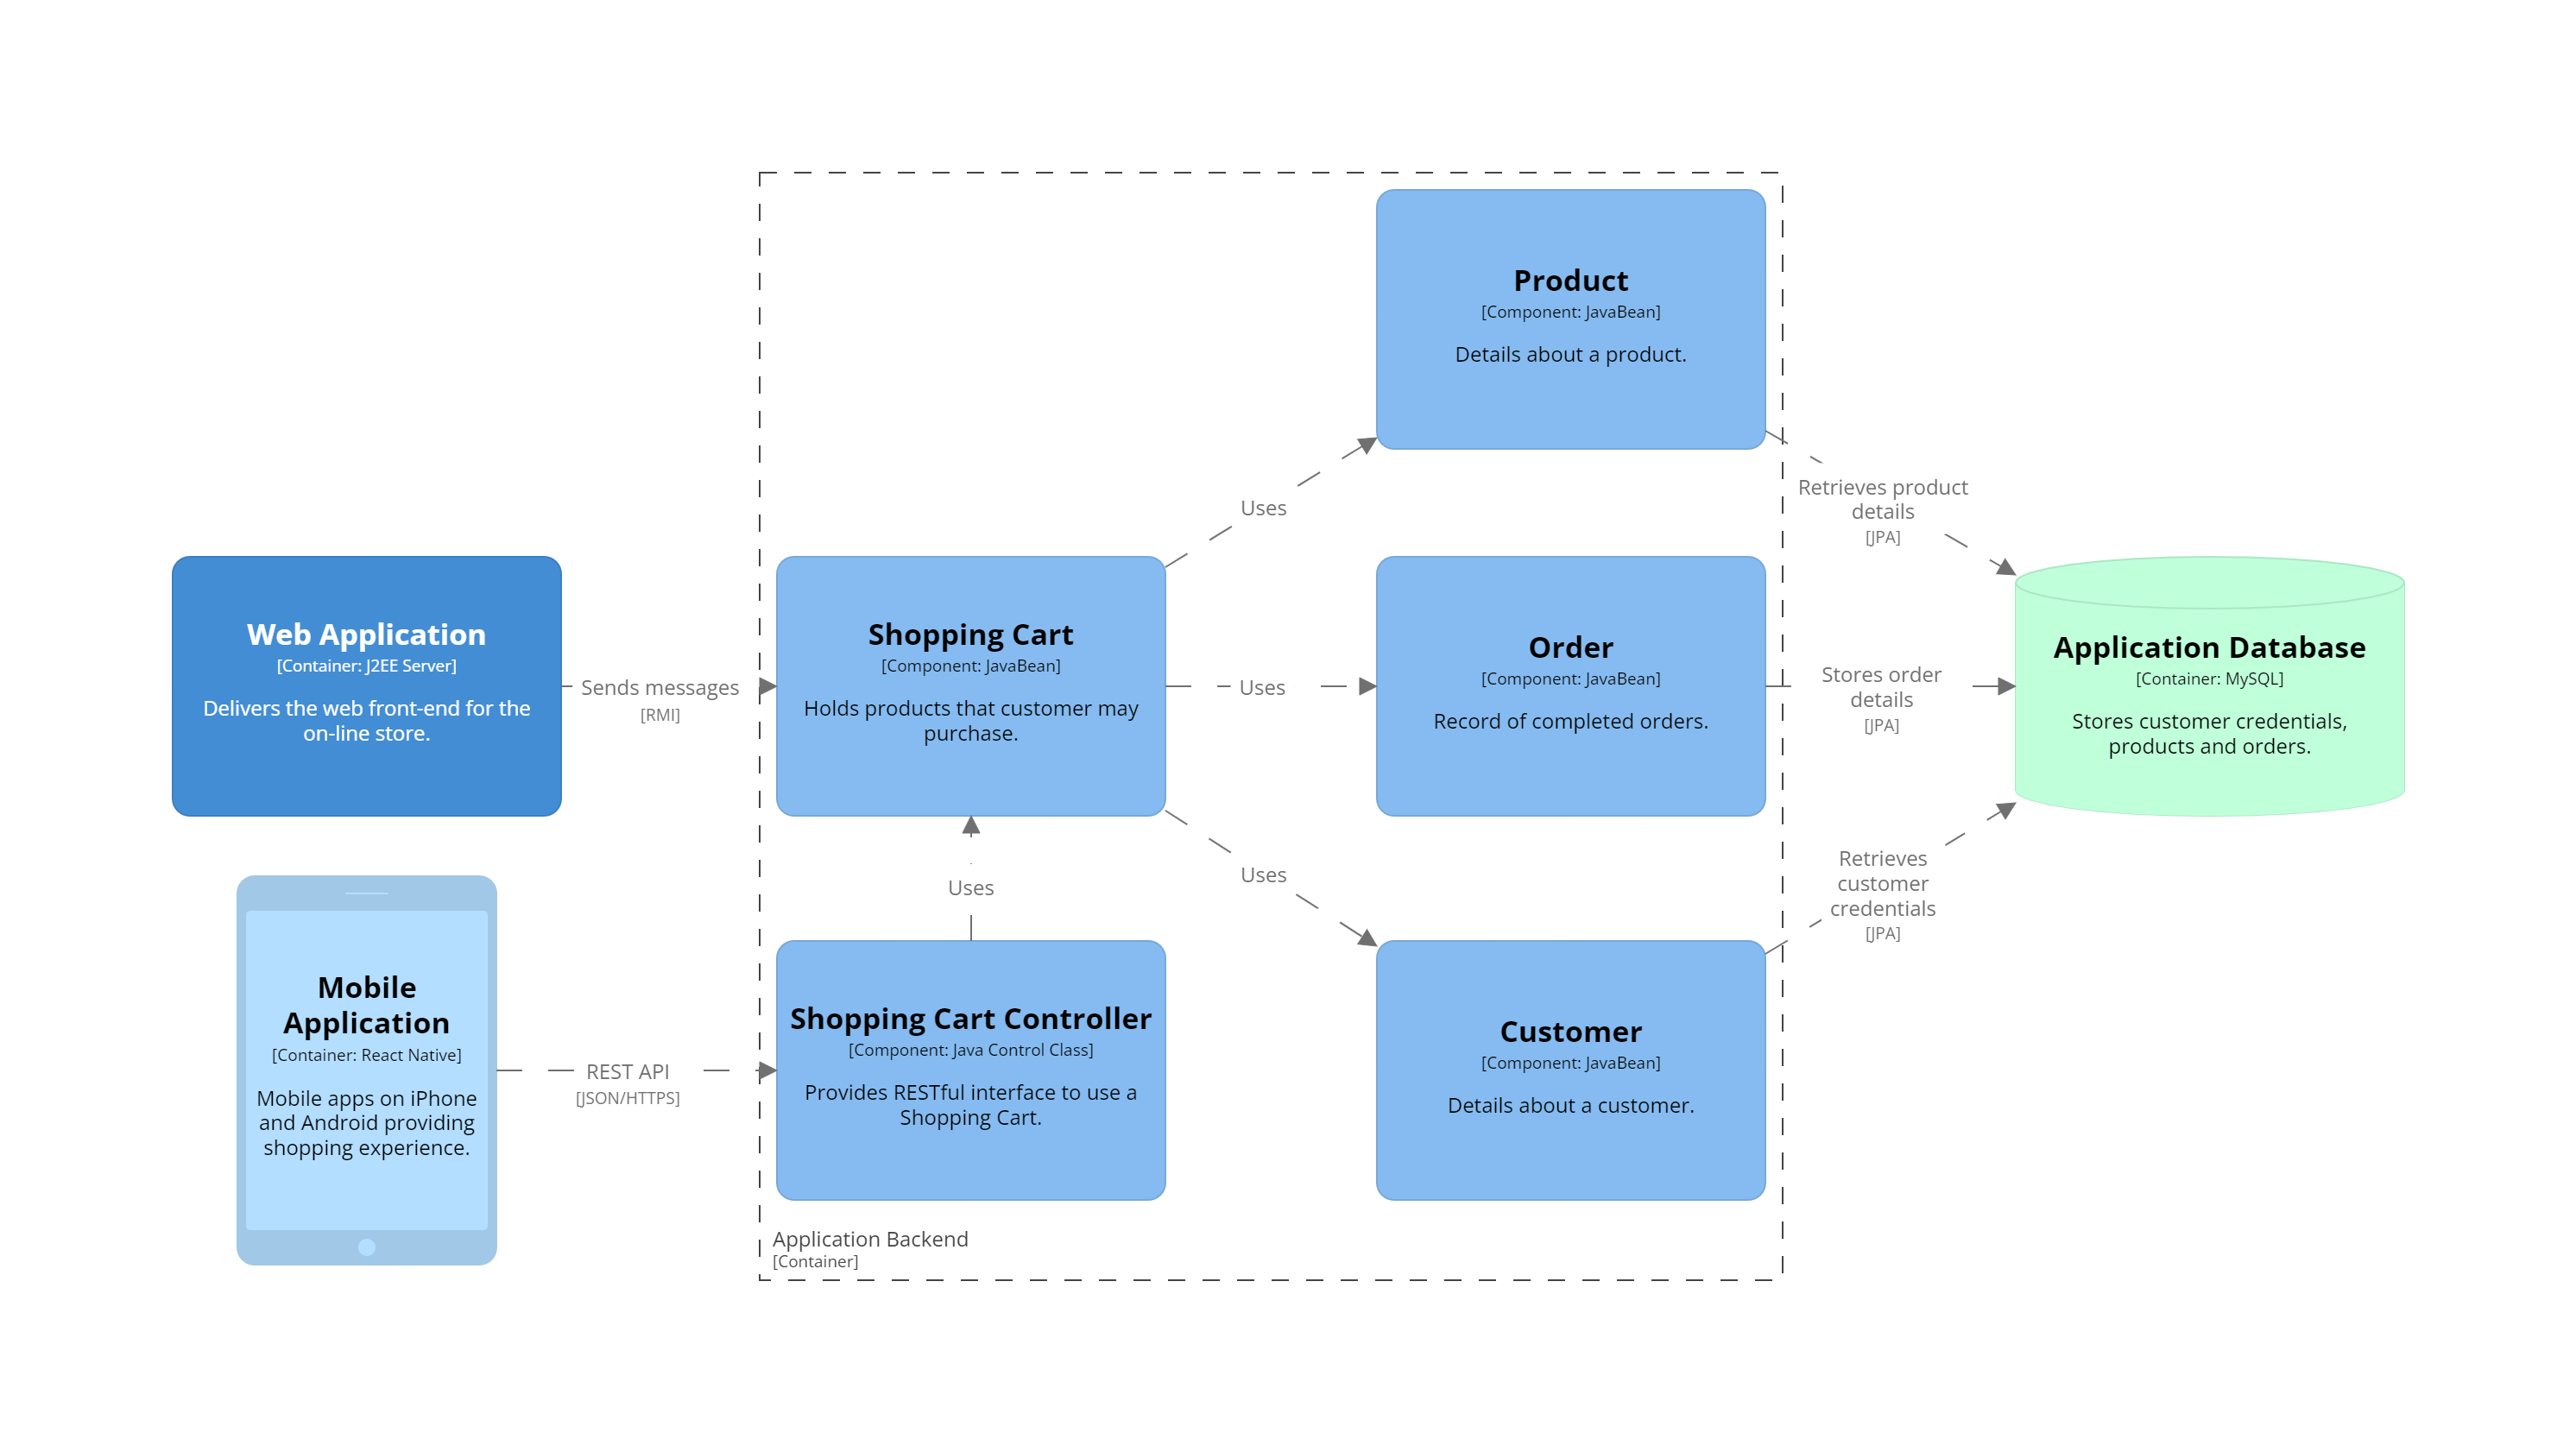
\includegraphics[trim=-550 185 197 40,clip,width=1.03\paperwidth]{../../notes/views/images/c4/appbackend_component_diagram.png}}}
\begin{frame}{C4 Model: Components}
    \centering
    \vspace{71mm}
    \LARGE{\highlight{Elements} that implement a container}
\end{frame}
}
\note[itemize]{
    \item \highlight{Components} are the major parts/elements of a container
    \item Diagram shows how the components are \highlight{connected}
    \item Highlight key \highlight{technologies} used to implement components and communication
    \item Components typically have \highlight{interfaces}
}


\begin{frame}{C4 Model: Code}
    \begin{adjustwidth}{-10mm}{-10mm}
    \centering
    \vspace{3mm}
    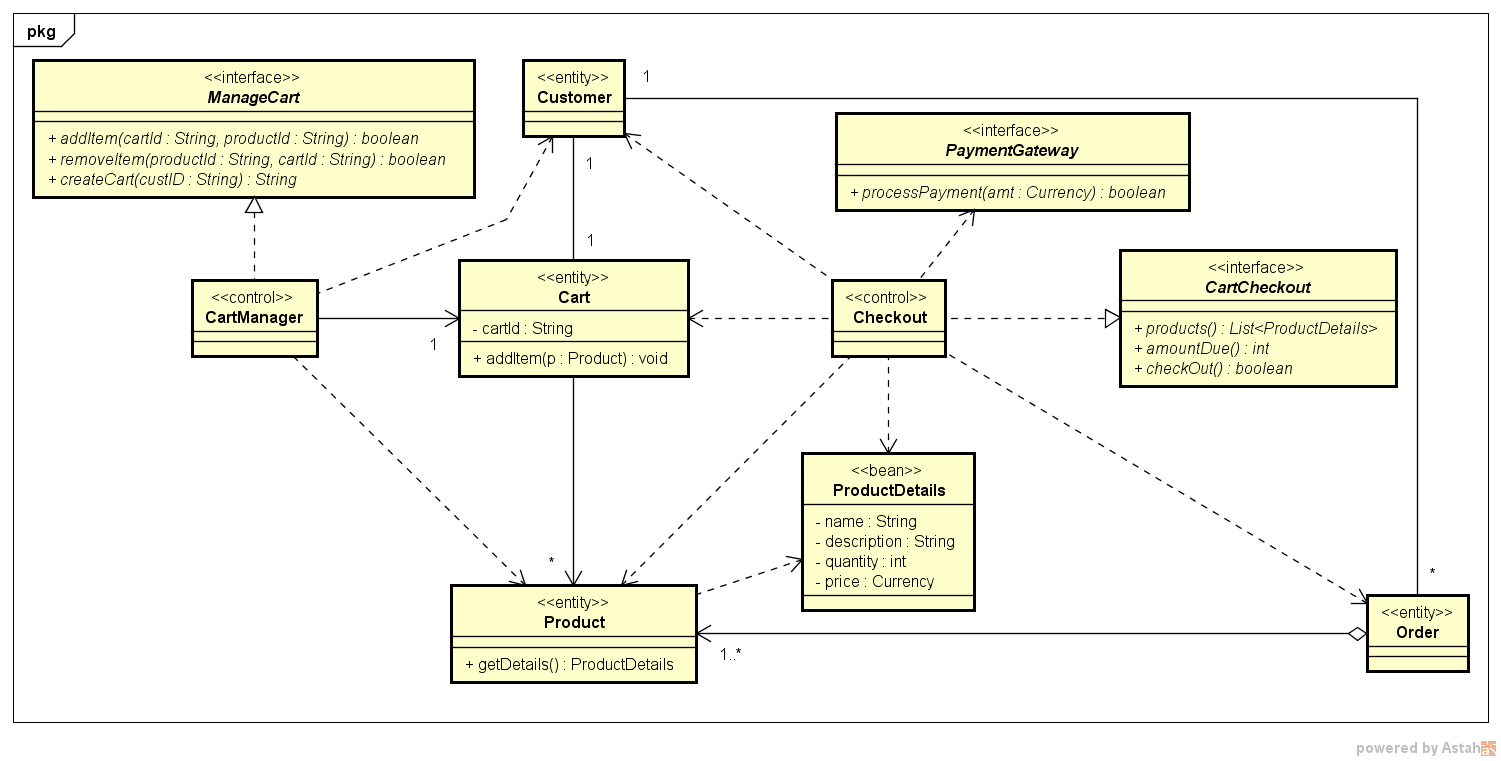
\includegraphics[trim=22 43 22 44,clip,width=0.98\paperwidth]{../../notes/views/images/uml/shopping_cart_class_diagram.png}
    \LARGE{\highlight{Structure} of code implementing a component}
	\end{adjustwidth}    
\end{frame}
\note[itemize]{
    \item UML \highlight{class diagram} of code structure
    \item C4 does not have code level diagrams
    \item \highlight{Often} they are not needed
    \item Can use UML, or others, if needed
}


\begin{frame}{C4 Model: Dynamic}
	\centering
    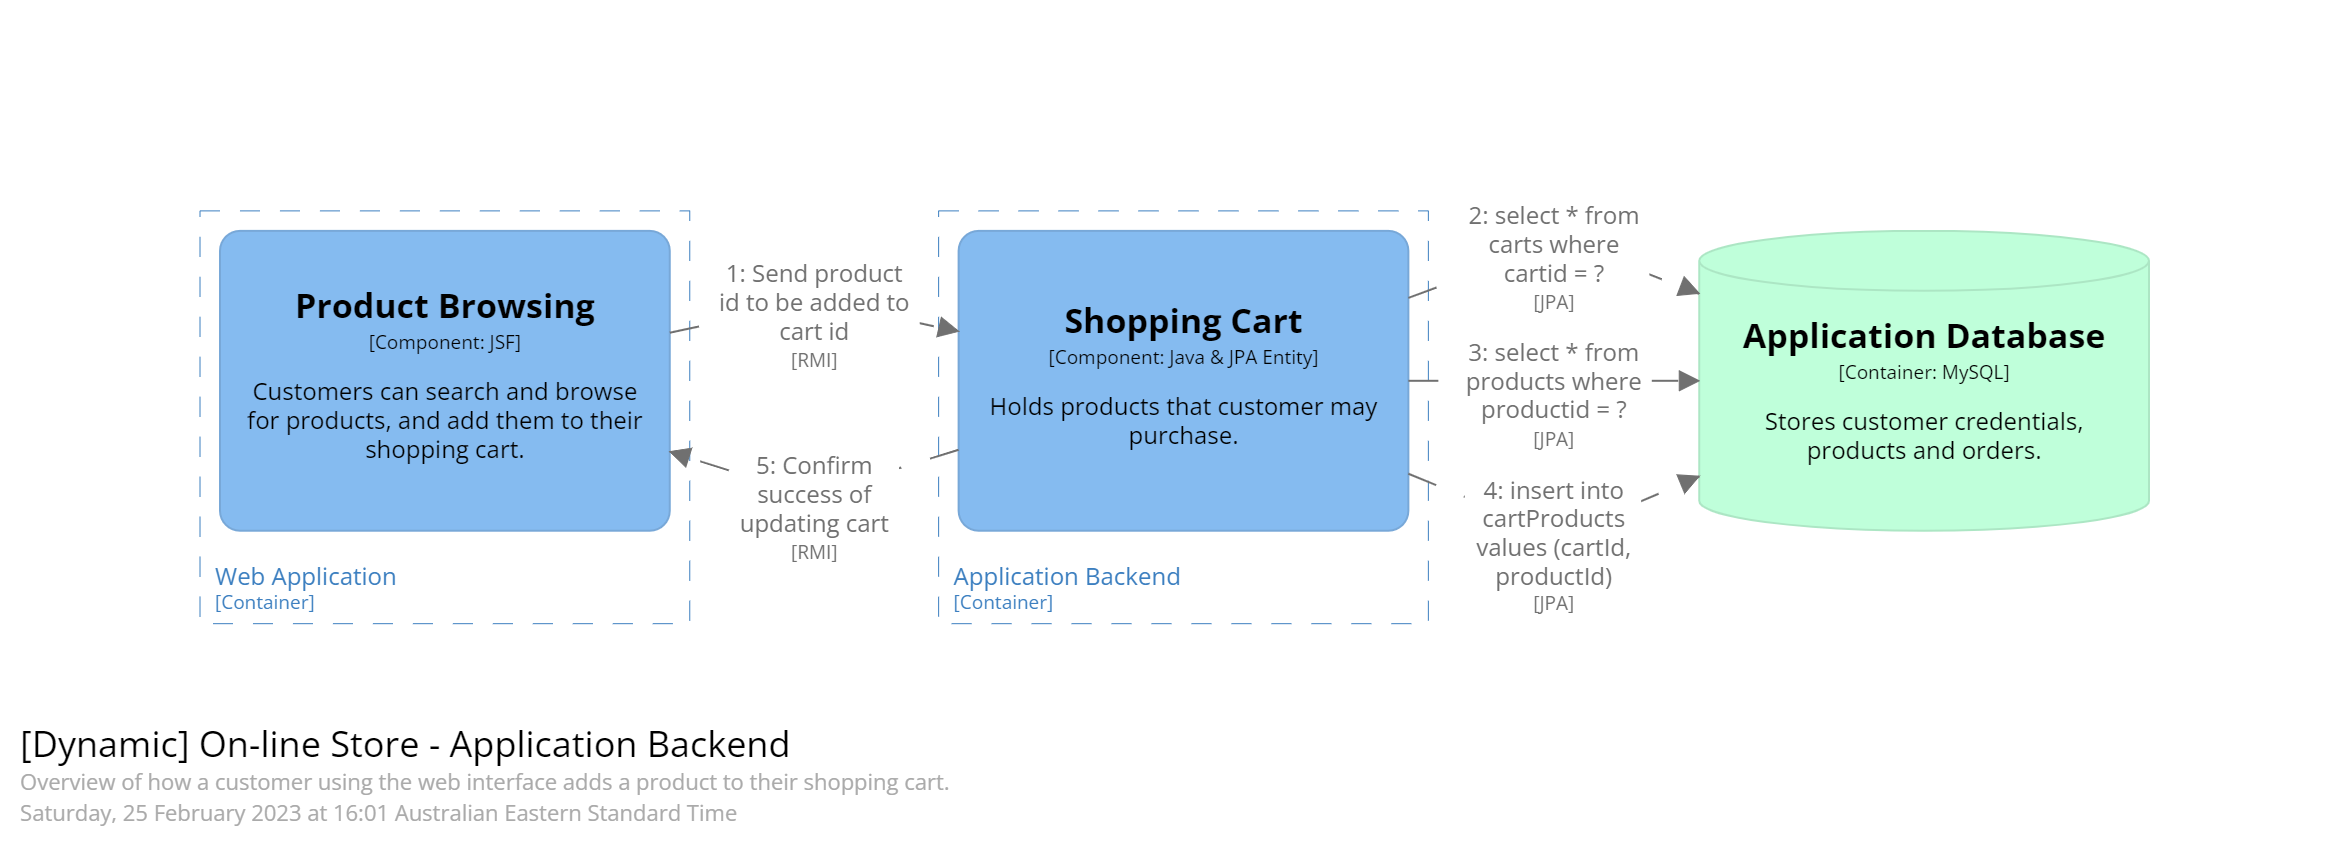
\includegraphics[trim=175 220 197 185,clip,width=0.75\paperwidth]{../../notes/views/images/c4/add_to_cart_dynamic_diagram.png}
    
    \vspace{1cm}
    \LARGE{How parts of the model \highlight{collaborate} to deliver \highlight{behaviour}}
\end{frame}
\note[itemize]{
    \item Focus on architecturally \highlight{significant} requirements
    \item What is not clear from other diagrams
    \item e.g. Complex interactions, concurrency, latency constraints, ...
    \item Can use UML sequence diagrams if more detail or formality is needed
}


{
\usebackgroundtemplate{\centerline{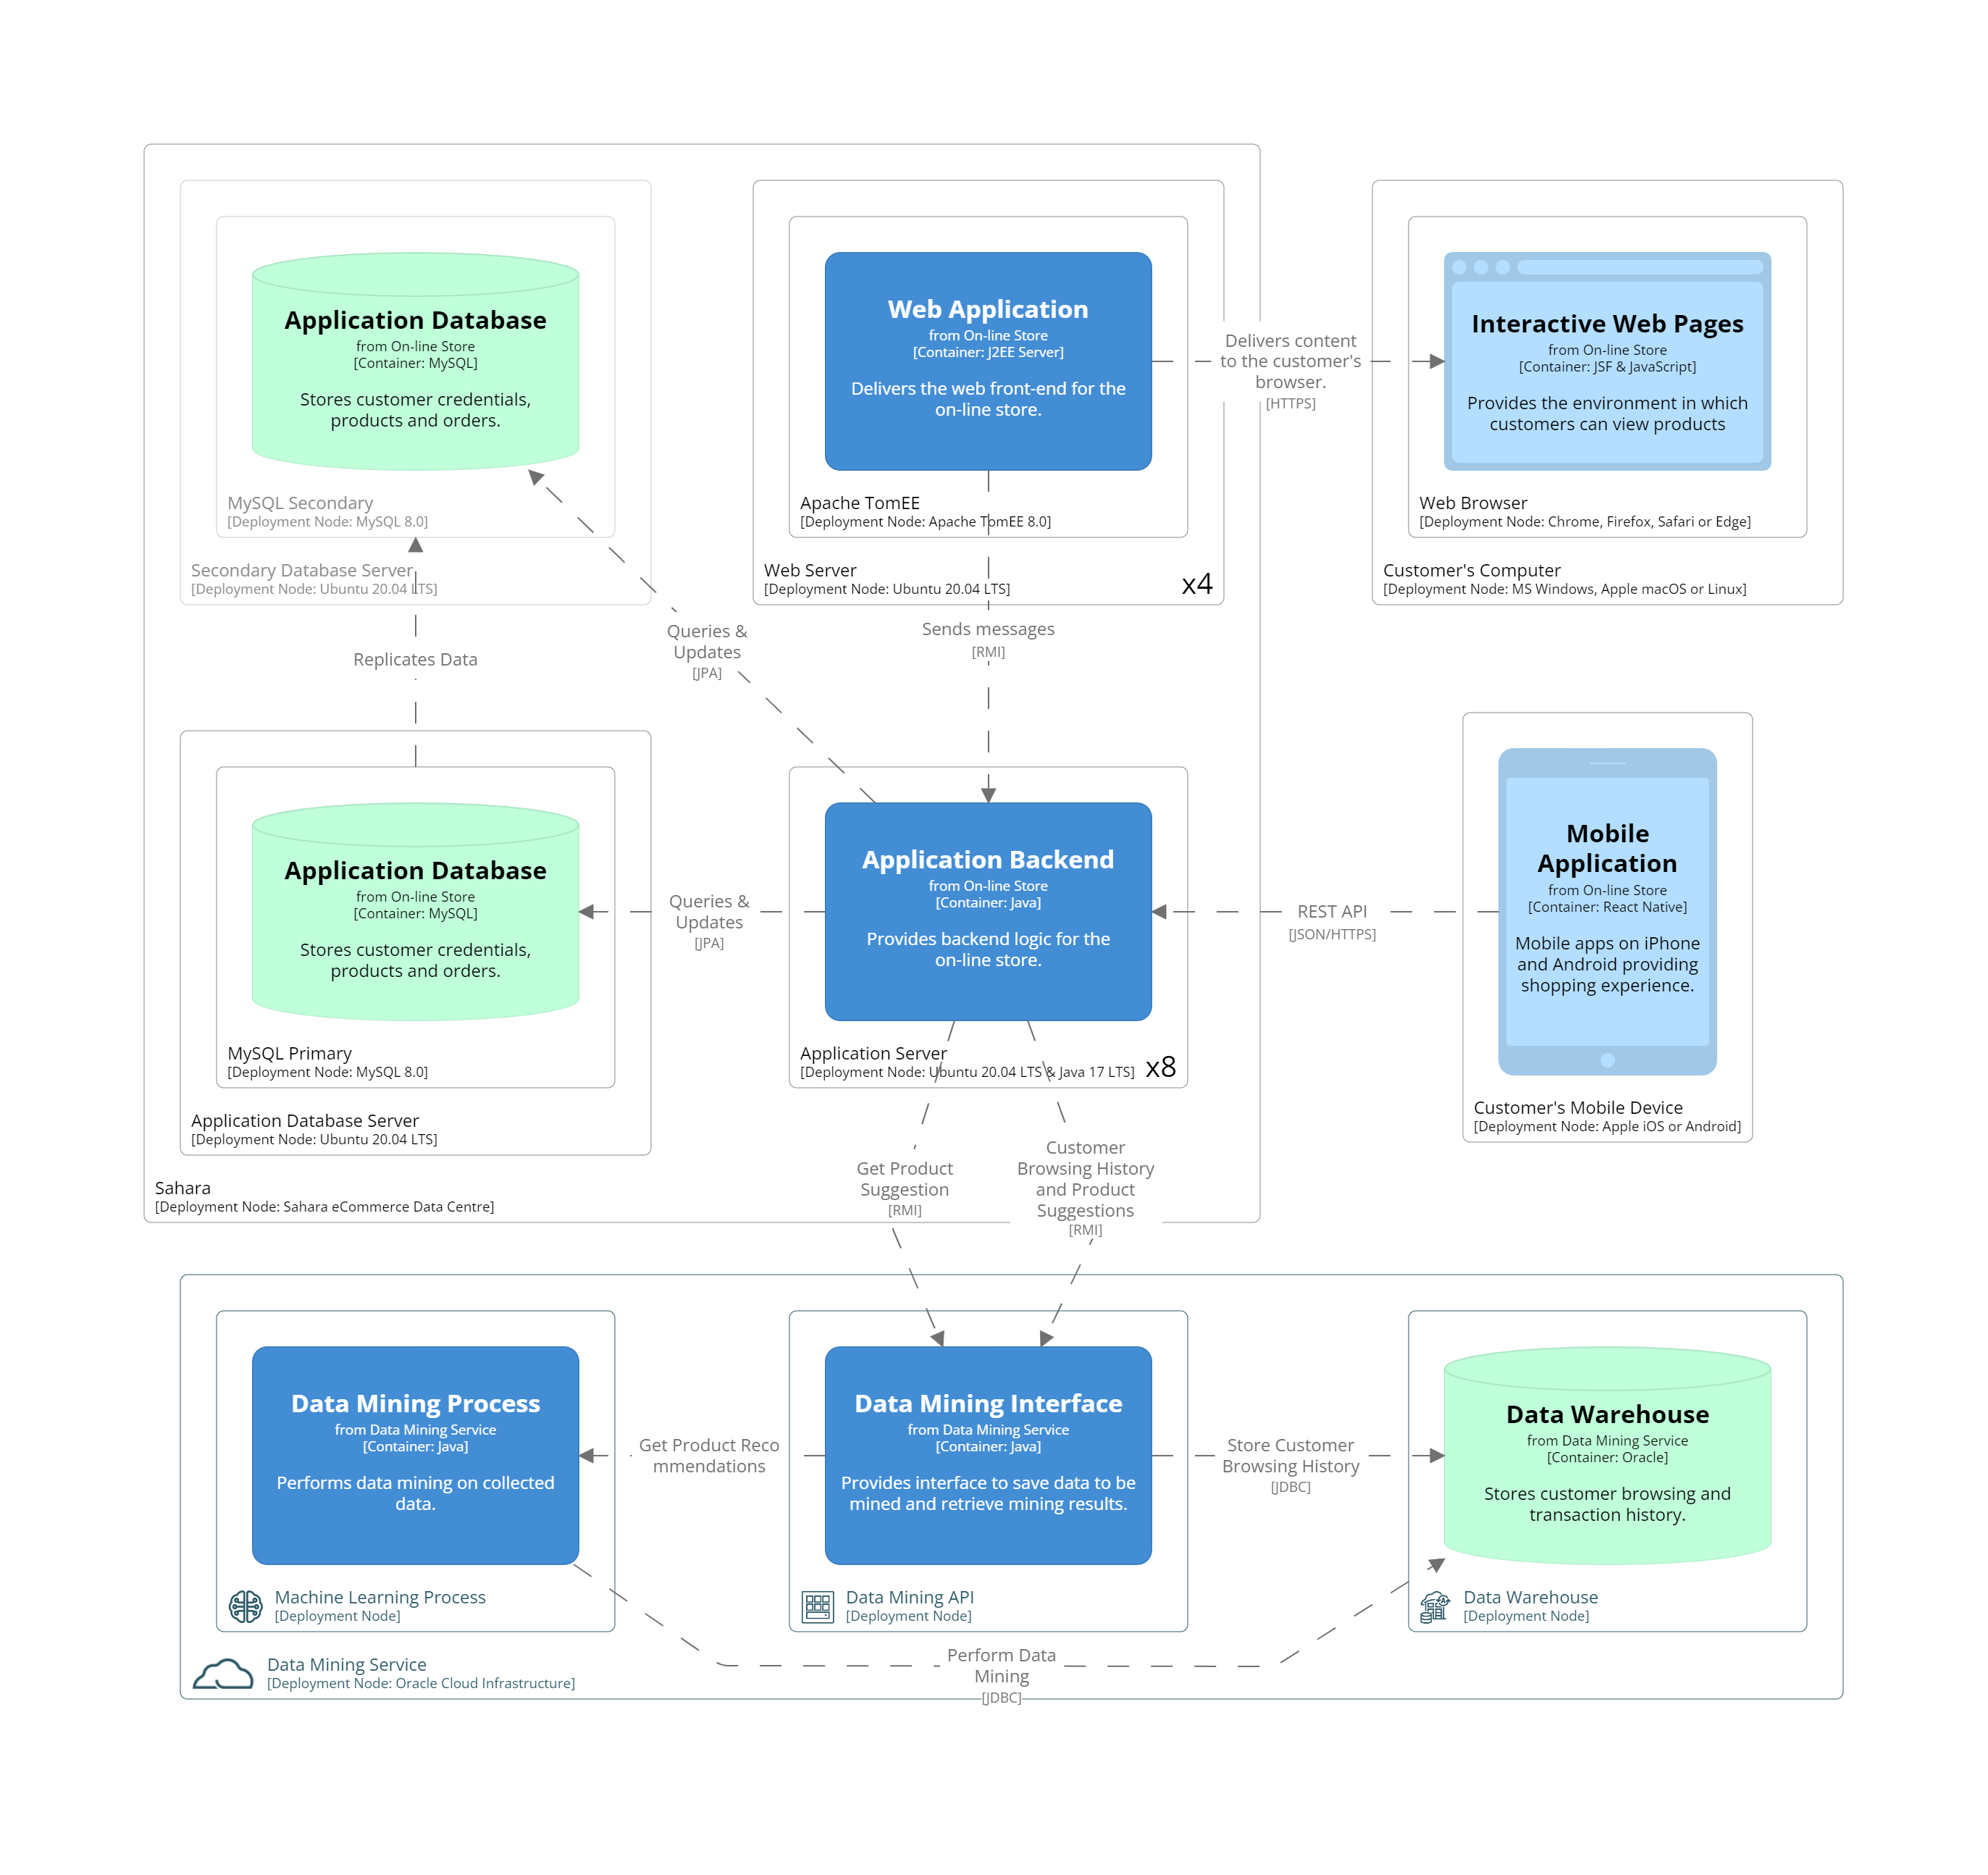
\includegraphics[trim=-750 850 195 100,clip,width=1.03\paperwidth]{../../notes/views/images/c4/deployment_diagram.png}}}
\begin{frame}{C4 Model: Deployment}
    \centering
    \vspace{71mm}
    \LARGE{\highlight{Infrastructure} on which system will be deployed}
\end{frame}
}
\note[itemize]{
    \item \highlight{Physical} architecture
    \item Which \highlight{containers} run on what \highlight{platforms} (\textit{deployment nodes})
}


%\begin{frame}{C4 Model}
%\Large{
%\begin{description}
%    \item<1->[Context] ~~~~
%    \begin{itemize}
%        \large{\item[$\bullet$] How software system fits into broader \highlight{environment}}
%    \end{itemize}
%    \item<2->[Structure] -- Containers, Components, Code
%    \begin{itemize}
%        \large{\item[$\bullet$] \highlight{Levels} of detail}
%    \end{itemize}
%    \item<3->[Behaviour] -- Dynamic
%    \begin{itemize}
%        \large{\item[$\bullet$] How elements \highlight{interact} to deliver features}
%    \end{itemize}
%    \item<4->[Infrastructure] -- Deployment
%    \begin{itemize}
%        \large{\item[$\bullet$] How system is \highlight{deployed} on computing platforms}
%    \end{itemize}
%\end{description}
%}
%
%\end{frame}
%\note[itemize]{
%    \item No code level diagrams -- Use others like UML class diagrams
%    \item UML sequence as alternative to C4 dynamic diagrams
%}


\begin{frame}{4+1 Views}

\Large{
\begin{description}
    \item<1->[Logical] -- \highlight{Structure} of how the software is implemented
    \begin{itemize}
        \large{\item[$\bullet$] components/classes, relationships, interactions}
    \end{itemize}
    \item<2->[Process] -- \highlight{Dynamic} behaviour
    \begin{itemize}
        \large{\item[$\bullet$] concurrency \& distribution, fault tolerance, process control, ...}
    \end{itemize}
    \item<3->[Development] -- \highlight{Organisation} of the software in the development environment
    \item<4->[Physical] -- \highlight{Map} executable software containers to hardware
    \begin{itemize}
        \large{\item[$\bullet$] address non-functional requirements}
        \begin{itemize}
            \item[$\bullet$] availability, reliability, scalability, throughput, ...
        \end{itemize}
    \end{itemize}
    \item<5->[Scenario] -- \highlight{Demonstrate} functionality delivered by architecture
    \begin{itemize}
        \large{\item[$\bullet$] use case details}
        \begin{itemize}
            \item[$\bullet$] \highlight{drive} functional design of architecture
            \item[$\bullet$] \highlight{validate} design of architecture
            \item[$\bullet$] \highlight{illustrate} purpose of architecture
        \end{itemize}
    \end{itemize}
\end{description}
}

\end{frame}


\point[\LARGE{Reading...}]{``Architectural Views'' Notes\footnote{Remember, I said you had to read the notes.} \cite{view-notes}}


\references{articles,books,ours}

\end{document}